\newpage
\section{Solutions techniques} % (10 pages) Solutions techniques mises en oeuvre

%synthèse de l'existant (couverture fonctionnelle existante (architecture logicielle par ex.), contraintes inhérentes au projet (outils, librairies, …), s'appuyant sur une bibliographie précise

%description de la (ou des) solution(s) envisagée(s) et des outils qui seront utilisés

%protocole d'évaluation envisagé pour valider votre solution ou mesurer son efficacité

\subsection{Synthèse de l'existant} % (objectif perso : 4 pages)
\subsubsection{Architecture logicielle}
\label{sec:architecture}
\paragraph*{Architecture 3-tiers\\}
Topaze web est bâti selon une architecture 3-tiers : 
\begin{sitemize}
\item la \textit{couche présentation} qui sert à l'affichage des informations et qui tourne sur le navigateur du client.
\item la \textit{couche métier} qui contient la logique applicative.
\item la \textit{couche d'accés aux données} qui garantie la persistance des données (base(s) de données). 
\end{sitemize}

\paragraph*{Les utilisateurs\\}
Le projet Topaze Web aura deux types d'utilisateurs : 
\begin{sitemize}
\item \textit{Les infirmiers, kinésithérapeutes et autres professionnels de la santé} qui utiliseront Topaze au quotidien pour la gestion des feuilles de soins, de la facturation, des dossiers patients etc. 
\item \textit{Le service technique d'IDEA} (la société soeur de Supralog qui commercialise Topaze) : qu’il s’agisse des personnes
chargées d’administrer les comptes utilisateurs et cabinets ou les personnes étant au SAV, ils
utiliseront l’application pour gérer les abonnements et répondre aux problèmes techniques des
clients finaux.
\end{sitemize}

Pour résumer, voici une schéma de l'architecture 3-tiers de Topaze Web :
\begin{figure}[H]
	\vspace{-10pt}
  \centering
  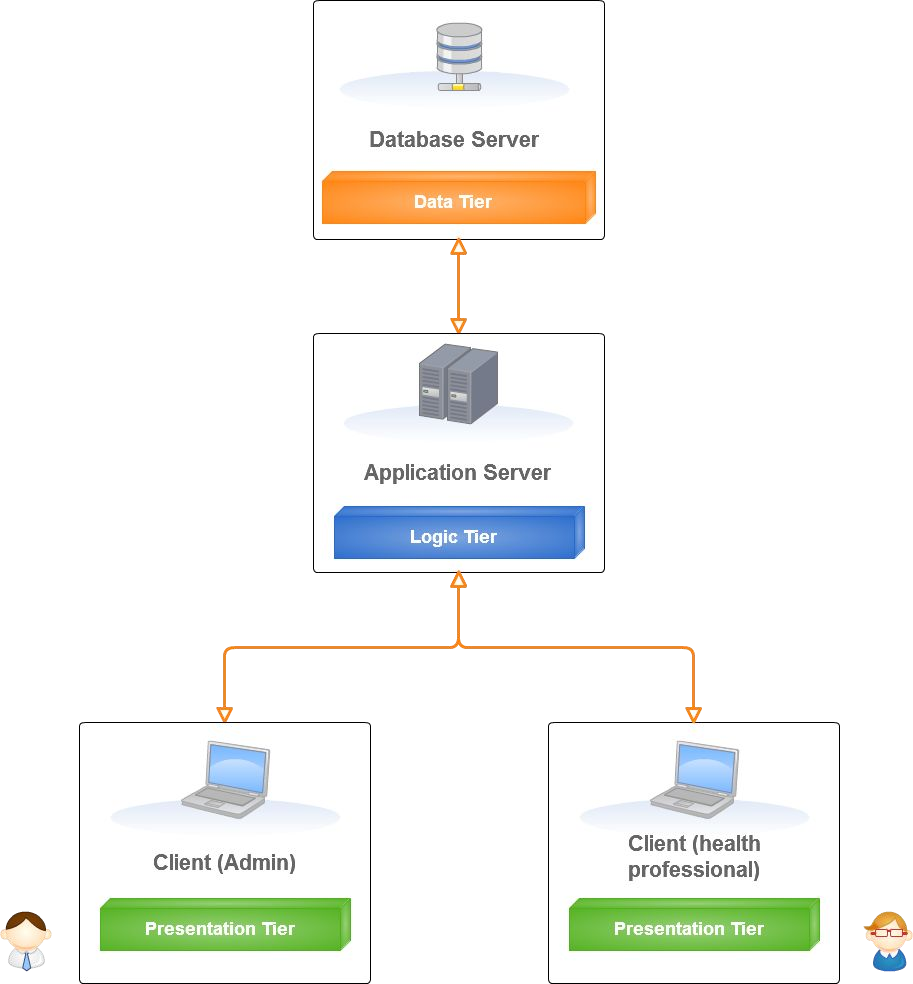
\includegraphics[width=8cm]{./img/architecture1}
  \caption{\label{fig:mb_va_ast} Schéma de l'architecture 3-tiers (créé par Tom Veniat, utilisé avec son accord)}
\end{figure}

Afin de satisfaire les besoins de ces deux types d'utilisateurs, deux applications qui accèdent aux mêmes données ont été crées: 

\begin{sitemize}
\item \textit{Topaze} : l'application utilisée par les professionnels de la santé. 
\item \textit{Opale} : l'application utilisée par les administrateurs.
\end{sitemize}

\paragraph*{L'application Topaze\\}
L'application Topaze a été scindée en deux parties : \textit{Topaze REST} et \textit{Topaze Webapp}.\\
\textit{Topaze Rest} est un serveur REST, à accès sécurisé par token. Il réalise les opérations liées à la logique métier et il fait persister les données en base. Topaze Rest est réalisé grâce au framework Spring MVC \cite{bib:spring}\\
\textit{Topaze Webapp} utilise JSF pour mettre les données en forme avant affichage \cite{bib:jsf}. Son accès est sécurisé via une authentification par sessions. Elle contacte \textit{topaze REST} afin de rapatrier les données, puis elle les met en forme avant de les envoyer au client (le navigateur).

\paragraph*{L'application Opale\\}
Opale et Topaze ont une base de données en commun. De cette manière, un administrateur d'Opale peut ajouter un utilisateur qui sera ensuite utilisable dans Topaze. \\
Les deux applications sont séparées car elles sont utilisées par des utilisateurs différents, mais également parce qu'elles effectuent des tâches de nature différente. En effet, les tâches réalisées par les administrateurs, dans Opale, se résument à des opérations CRUD \footnote{CRUD: Create, Read, Update, Delete} sur la base de données. Dans Opale, il n'y a donc pas ou peu de logique métier. 
De ce fait, le code de l'application Opale est presque entièrement générée au moyen du \textit{Skeleton Generator}.\\ \\
Le \textit{Skeleton Generator} est un projet open-source, développé par le chef de projet, qui permet de faire du M2C \footnote{M2C: Modèle To Code}. Dans opale, on décrit donc les modèles de données via un fichier XML (cf annexe \ref{fig:xml}), puis le générateur est utilisé pour créer les entités en base de données, générer le code des DAO \footnote{DAO: Data Access Object} qui serviront pour Opale et Topaze et générer tout le code d'Opale (les composants-métier, les objets métiers, les services, l'api rest, ainsi que l'application web). 

\paragraph*{L'application Sesame\\}

La manipulation des Feuilles de Soins Electroniques (FSE) et la facturation nécessitent la lecture d'informations présentes sur la carte vitale du patient. D'autre part, les logiciels utilisant les FSE sont soumis à l’obtention d’un agrément délivré
par les représentants des organismes d’Assurance Maladie. Cet agrément est obtenu après de
nombreux tests vérifiant que le logiciel en question respecte un cahier des charges très précis.\\
La gestion de la facturation et des FSE étant nécessaire à l’application, mais pouvant
être externalisée, c’est une troisième application qui en a la responsabilité. \\
Cette troisième application nommée \textit{Sesame} répond à trois problématiques : 
\begin{sitemize}
\item La communication avec le lecteur de cartes vitales.
\item La facturation des actes réalisés par les praticiens, en fonction des informations du patient présentes sur la carte vitale.
\item La communication avec Topaze et la restriction des accés à la carte vitale.
\end{sitemize}

Afin de pouvoir communiquer avec la carte vitale un driver doit être installé sur la machine de l'utilisateur. Par la suite, le serveur Sesame communique avec le driver via des websockets afin d'avoir accès aux informations de la carte vitale.

\paragraph*{Schéma d'architecture global\\}
Voici le schéma d'architecture globale représentant l'architecture 3-Tiers et la communication entre les différentes applications :
\begin{figure}[H]
  \centering
  \centerline{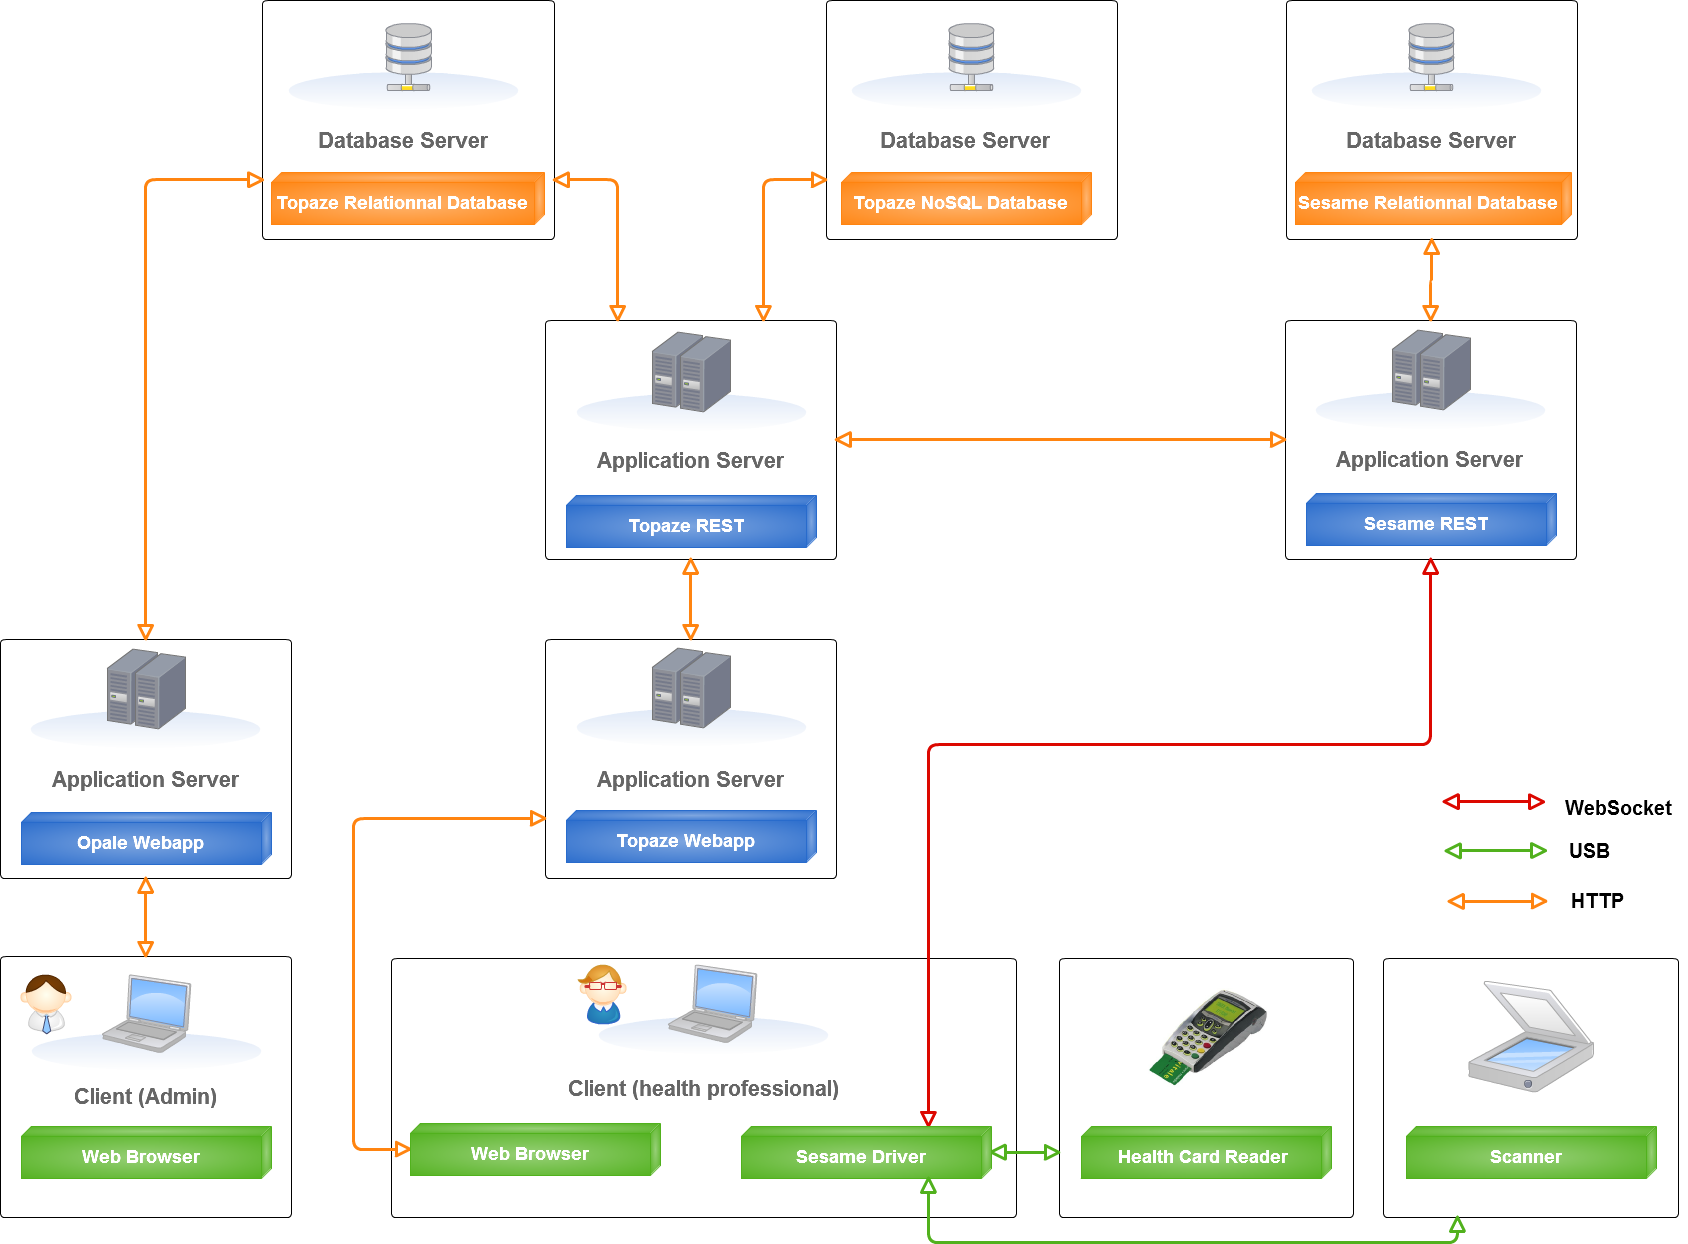
\includegraphics[width=20cm]{./img/architecture5}}
  \caption{\label{fig:mb_va_ast} Schéma d'architecture global (créé par Tom Veniat, utilisé avec son accord)}
\end{figure}

\subsubsection{Technologies utilisées}
Les technologies utilisées par le projet sont :
\begin{sitemize}
\item Bases de données : PostgreSQL pour les modèles de données, MongoDB et GridFS pour les fichiers.
\item ORM : Hibernate\cite{bib:hibernate}
\item Serveur : Tomcat
\item Backend : Java8\cite{bib:java8} et Spring\cite{bib:spring}
\item Front-End : JSF\cite{bib:jsf} et Primefaces
\end{sitemize} 

\subsection{Solution envisagée}
\subsubsection{Conception et implémentation du dossier médical}

%\item Analyse de l'existant (fonctionnalités et comportements de Topaze Maestro) 
%\item Etude de la faisabilité des différentes fonctionnalités.
%\item Discussion du besoin avec le chef de projet et/ou la maitrise d'ouvrage.
%\item Proposition d'une solution qui réponde fonctionnellement au besoin.
%\item Spécification  du model métier (entités de la base de données) qui réponde au besoin.
%\item Spécification de l'API Rest.
%\item Spécification des interfaces graphiques si besoin.
%\item Implémentation de la solution (backend + frontend) dans Topaze Web.
\paragraph{Analyse de l'existant\\}
Le dossier médical de Topaze Web doit, si possible, apporter les mêmes fonctionnalités que celui présent dans Topaze Maestro.
La première étape de conception a donc consisté à faire une analyse de l’existant et à lister les fonctionnalités présentes (il s’agit de la liste décrite dans la section Problématique).

\paragraph{Etude de la faisabilité\\}
Ensuite, j'ai étudié la faisabilité des différentes fonctionnalités et les ai triées en fonction de leur difficulté à être implémentées en web. La plupart des fonctionnalités peuvent être créées sans difficulté, cependant certaines ont soulevé des questions :

\subparagraph*{Le cas des objets OLE} est particulier, car il s'agit là d'un protocole de Microsoft à destination de Windows. 
Il ne peut donc pas être utilisé dans une solution web. À ce niveau, il était donc nécessaire de savoir quels types d'objets devaient être supportés et si la fonctionnalité était vraiment importante. En effet, chaque objet à supporter nécessite de batir une solution sur mesure.\\
Après discussion avec le chef de projet, il a été décidé que l'utilisation des objets OLE ne serait pas géré à proprement parlé dans l'application. Cependant, l'utilisateur peut, s'il le désire, télécharger différents types de fichiers sur l'application et les récupérer ensuite pour les éditer avec ses propres logiciels.

\subparagraph*{Le cas des documents RichText} a lui aussi demandé un traitement spécifique. Dans Topaze Maestro, les documents au format richtext peuvent être téléchargés puis édités directement depuis l'application. En web, l'édition de documents au format richtext n'est pas habituelle. En revanche, de nombreux éditeurs \gls{WYSIWYG} existent et permettent d'éditer du Markdown, du BBCode ou du HTML. J'ai donc choisi d'intégrer un composant extérieur afin de remplir cette tâche. Afin que les utilisateurs de Topaze Maestro puissent réutiliser leurs données dans Topaze Web, il a été décidé que les fichiers au format RTF seraient transformés en HTML au moyen d'un traitement batch en cas de migration de donnée. \\
Les choix techniques et l'intégration du composant seront décrits dans la section \ref{editeur_section}.

\subparagraph*{Le cas des sons} est particulier. Pendant longtemps, cette fonctionnalité a été implémentée en web en utilisant du flash. Aujourd'hui, la balise audio d'HTML5 permet de lire des sons de façon native dans les navigateurs. Cette fonctionnalité d'HTML5 est supporté par quasiment tous les navigateurs, sauf IE8 \footnote{Support de la balise audio : http://caniuse.com/\#feat=audio}. \\
En ce qui concerne l'enregistrement des sons (possible dans Topaze Maestro via un objet OLE), HTML5 offre l'API getUserMedia qui permet d'accéder au flux audio ou vidéo d'un périphérique externe. Cependant, le support de cette fonctionnalité n'est pas encore assuré par tous les navigateurs \footnote{Support de l'API getUserMedia : http://caniuse.com/\#feat=stream}. Afin de résoudre la question du support des navigateurs, des bibliothèques open-source telles que \textit{getUserMedia.js}\footnote{getUserMedia.js : https://github.com/addyosmani/getUserMedia.js} ont été développées. Ces bibliothèques utilisent la getUserMedia API si elle est disponible et utilisent Flash si ce n'est pas le cas.

\paragraph{Elaboration d'une solution\\}
Afin d'élaborer une solution, j'ai commencé par réaliser un diagramme de classe d'analyse modélisant les différents objets qui interviennent dans le dossier médical:

\begin{figure}[H]
  \centering
  \includegraphics[width=11cm]{./img/class}
  \caption{\label{fig:mb_va_ast} Diagramme de classe d'analyse du dossier médical.}
\end{figure}

Dans ce diagramme d'analyse, on peut voir que le dossier médical est constitué de deux types de documents : ceux que j'ai appelé les "Documents MIME" qui correspondent à des fichiers binaires (sons, images, textes) et les autres, qui sont des objets métiers manipulés dans l'application.\\

Une fois ce diagramme réalisé s'est posée la question de la persistance des données. Avant toute chose, j'ai regardé le contenu de la base de données afin de savoir quelles entités étaient déjà présentes.\\
Voici le modèle conceptuel de la base de données au départ (seules les entités concernant le cas étudié ont été représentées)  :

\begin{figure}[H]
  \centering
  \includegraphics[width=15cm]{./img/existing_model}
  \caption{\label{fig:mb_va_ast} Modèle UML conceptuel de la base de donnée, au départ.}
\end{figure}

Dans la base de donnée, les prescriptions étaient déja présentes. Il restait donc à ajouter les documents issus de fichiers. \\
Voici donc l'ajout que j'ai réalisé au modèle de donnée : 
\begin{figure}[H]
  \centering
  \includegraphics[width=13cm]{./img/created_model}
  \caption{\label{fig:mb_va_ast} Modèle UML illustrant les ajouts à la base de données.}
\end{figure}

Ensuite, s'est posée la question du stockage du contenu des fichiers. Deux choix étaient possibles : les stocker en base, ou directement dans un système de fichier. Cette question s'était déjà présentée plus tôt dans le projet, et l'équipe avait décidé de stocker les données binaires dans une base de données Mongo DB munie de GridFS. Ce choix a été fait pour les caractéristiques de disponibilité et de scalabilité propre à MongoDB.\\
La base de données PostgreSQL est donc utilisée pour stocker les méta données liées au fichier et leur contenu est stocké dans MongoDB. Lorsqu'on a besoin du contenu d'un fichier, on récupère son id dans Postgre et l'on fait une requête dans MongoDB pour obtenir son contenu. La convention choisie est que le filename dans Mongo correspond à l'id du document dans Postgre. \\

Dans MongoDB, deux collections sont utilisées, par défaut, par GridFS pour stocker les fichiers :  
\begin{figure}[H]
  \centering
  \includegraphics[width=12cm]{./img/gridfs}
  \caption{\label{fig:mb_va_ast} Collections utilisées par GridFS pour le stockage des fichiers.}
\end{figure}
La collection \textit{Chuncks} sert à stocker les données du fichier et la collection \textit{Files} sert à stocker les méta-données du fichier.

\paragraph{Phase d'implémentation\\}
Une fois le modèle de données mis en place, il ne reste plus qu'à réaliser l'implémentation dans Topaze Rest et \textit{Topaze Webapp}. 
À ce niveau, différentes classes sont à implémenter dans la \textit{Topaze Webapp} et dans \textit{Topaze Rest}. Afin de comprendre quelles classes sont à implémenter, voici un schéma illustrant la requête permettant d'obtenir le dossier médical (le diagramme est également fourni en plus grand, en annexe \ref{fig:diag_seq}, pour les lecteurs sur papier):
\begin{figure}[H]
  \centering
  \includegraphics[width=17cm]{./img/diag_seq}
  \caption{\label{fig:mb_va_ast} Diagramme de séquence modélisant la requête du dossier médical.}
\end{figure}

Comme on peut le voir, l'architecture de la \textit{webapp} suit un modèle MVC. Du côté de \textit{Topaze Rest}, il y a plusieurs packages : 
\begin{itemize} 
\item \textit{API} qui définit les services et les modèles (qui correspondent à des vues simplifiés des objets tirés de la base)
\item \textit{REST} qui définit les les contrôleurs (qui font le mapping entre une url et un service)
\item \textit{REST Client} qui définit des services clients utilisés par la web-app pour contacter les contrôleurs.
\item \textit{Business components} qui définit les objets tels que les mappers qui permettent de créer des vues ad-hocs à partir des modèles issus de la base de données.
\end{itemize}

Enfin, on utilise également les DAO \footnote{DAO: Data Access Object} définis dans Opale qui permettent d'obtenir les informations de la base de données.\\

Une capture d'écran du dossier médical de Topaze Web est disponible en annexe \ref{fig:dossier_web}.

\subsubsection{Choix et intégration de l'éditeur de texte}\label{editeur_section}
% Choix editeur + licence permissive et non contaminante
% Problème Richtext et données existantes

L’édition de texte est une fonctionnalité importante de Topaze Maestro. Il fallait donc qu’un éditeur soit implémenté ou intégré. De nombreux éditeurs de texte de qualité ont déjà étés développés et il en existe sous toutes les licences. Il a donc été choisi d’intégrer un composant existant. Cela permet d’avoir un composant robuste, bien documenté, éprouvé par toute une communauté et en continuelle évolution.\\

Les critères que j’ai pris en compte lors du choix étaient la notoriété du projet, le nombre de contributeurs et d’utilisateurs, son ancienneté, le support proposé, le nombre de fonctionnalités offertes, les possibilités de configuration, la possibilité de greffer de nouveaux plugins et enfin, la licence.\\

La licence était une question importante car Topaze Web est destiné à être commercialisé. Il n’était donc pas possible de choisir un éditeur distribué sous une licence à fort copyleft (par exemple la GPL). Un tel choix aurait contraint Topaze Web à être lui-même distribué sous licence GPL.\\

Pour finir, l’éditeur CKEditor a été choisi car il propose une licence LGPL, dispose d’une bonne communauté, de nombreux plugins et de la possibilité d’ajouter facilement ses propres plugins.

\subparagraph*{Intégration de l’éditeur\\}
L’intégration se fait très facilement en ajoutant la librairie de l’éditeur. Il ne reste plus ensuite qu’à gérer le flot de données qui circulent entre l’éditeur et l’application. Du javascript est utilisé pour gérer la sauvegarde lors du click sur le bouton ou périodiquement si l’utilisateur ne sauvegarde pas.\\

Par la suite d’autres modifications seront apportées (vue réaliste faisant apparaître les pages telles qu’elles seront imprimées, galerie d’image, import d’images).\\

Une capture d'écran de l'éditeur de texte de Topaze Web est disponible en annexe \ref{fig:editeur_web}.

\subsubsection{La bibliothèque d'images}
Dans Topaze Maestro, la bibliothèque d'images contient uniquement des images prédéfinies. Dans la version web, il a été décidé qu'elle puisse également contenir des images importées par l'utilisateur.\\
De manière à ce que la bibliothèque soit simple à gérer, nous avons décidé (le chef de projet et moi) de créer un gestionnaire de fichiers avec une arborescence de dossiers.

\paragraph*{Elaboration du modèle de données\\}
Lors de la conception du modèle, la contrainte suivante devait être prise en compte : \\
Lorsqu'un utilisateur supprime une image de sa bibliothèque, si celle-ci a été insérée dans un document, elle doit continuer d'y appraître. \\
Ainsi, il était nécessaire de séparer en base, l'apparition d'une image dans la bibliothèque de son stockage pour utilisation dans les documents texte. \\
J'ai donc créé le modèle suivant : 

%TODO : MCD des directory, userImageAddress, UserImage : vérifier si on met les ID ou pas ...
\begin{figure}[H]
  \centering
  \includegraphics[width=12cm]{./img/directory_entities_concept}
  \caption{\label{fig:mb_va_ast} Modèle UML conceptuel du système de gestion de fichiers.}
\end{figure}

\paragraph*{Spécification de l'API REST\\}
En ce qui concerne l'API REST, elle contient les opérations de CRUD\footnote{CRUD: Create Read Update Delete} sur les dossiers et leur contenu.
L'API expose donc les urls suivantes concernant les dossiers : 
%TODO : à vérifier.
\begin{itemize}
\item GET /account/models/directory/{directoryId}
\item DELETE /account/models/directory/{directoryId}
\item POST /account/models/directory
\end{itemize}

Concernant les images contenues, ont trouve :
\begin{itemize}
\item GET /account/models/directory/{directoryId}/picutre/{pictureId}/content
\item DELETE /account/models/directory/{directoryId}/picutre/{pictureId}
\item POST /account/models/directory/picutre
\end{itemize}

\paragraph*{Modèle de l'API\\}
L'API REST récupère les donneés de la base au moyen de DAOs\footnote{DAO: Data Access Object} et peuple des objets métiers qu'elle va ensuite retourner.\\

Pour la base de donnée, il était plus simple de stocker l'arborescence de façon ascendante (chaque fichier contient l'id du dossier parent). Mais, concernant les objets métiers (qui eux seront exposés), on souhaite que l'arborescence soit stockée de façon descendante, pour que leur usage soit naturel.
En effet, les objets métiers sont ensuite utilisés pour générer les vues en HTML. Dans ce cas, on a donc en général accés à un dossier et on souhaite obtenir la liste de ses fils. \\

Pour représenter ce type de modèle, on pense naturellement au design pattern composite \cite{bib:compositePattern} : \\
\begin{figure}[H]
  \centering
  \includegraphics[width=12cm]{./img/directory_entities_concept}
  \caption{\label{fig:mb_va_ast} Modèle UML de classes du système de fichiers, suivant le patron de conception composite.}
\end{figure}

Cependant, les objets retournés par l'API REST seront transmis par le réseau et devront donc être sérialisés. Hors, l'outil utilisé pour la sérialisation (Jackson), ne gère pas nativement le polymorphisme de java. \\
Le moyen utilisé pour pouvoir le faire quand même consiste à utiliser des annotations Jacksons, ou à inclure un champ "type" dans le json retourné par l'API. Cependant, ce choix est couteux car il impose des contraintes fortes sur le client utilisant l'API: l'usage de Jackson ou l'ajout d'un mécanisme particulier pour parser les objets reçus.\\

N'ayant que deux types d'objets, j'ai donc préféré briser l'héritage.

%TODO  OK: schéma du nouveau modèle. => NON c'est hiddeux ...

\paragraph*{Implémentation de la partie WebApp\\}
La webapp effectue des traitements assez standards. Elle effectue des appels aux services REST pour obtenir les dossiers et leur contenu et expose un certain nombre de méthodes utilisables par les vues JSF grâce un controlleur.
Le modèle utilisé par la webapp est rudimentaire car il ne fait qu'encapsuler les objets métiers obtenus de l'API REST et stocke en plus quelques variables d'états pour la vue.

\paragraph*{Spécification de l'interface graphique\\}
Avant d'implémenter la vue en JSF dans l'application, j'ai réalisé un prototype en HTML et javascript dans plunker.
Plunker est un éditeur en ligne pour le front-end. Il permet de faciliter la programmation fron-end en proposant un aperçu en temps réel, une inclusion de librairie simple, une gestion de version, un stockage privé du code et un partage simple et rapide du résultat avec un tiers.

Une fois que le résultat était satisfaisant, il a suffit de convertir une partie du HTML en JSF pour l'intégrer au code.

\paragraph*{Création d'un composant réutilisable\\}
Le gestionnaire de fichier utilisé pour la bibliothèque d'image a vocation à pouvoir être réutilisé à d'autres fin.
J'ai donc créé un composant réutilisable.

En JSF, plusieurs choix sont possibles pour créer des composants réutilisables : 
\begin{itemize}
\item Les \textit{Inclusions de code} : c'est la solution la plus rudimentaire. Elle consiste à extraire un morceau de code et à l'inclure ensuite en utilisant des \textit{<ui:include>} et \textit{<ui:param>}. Cette solution est adoptée lorsque le code inclus n'est pas ou peu paramétrable et n'a pas une sémantique trés forte (i.e. le code ne représente pas réellement un composant à lui seul).
\item Les \textit{Custom Tags} : il s'agit de la solution la plus légère lorsqu'on souhaite créer un composant réutilisable. C'est une méthode trés proche des inclusions de code, mais qui offre une interface plus propre. Elle permet une librairie de nouvelles balises jsf, qui peuvent accepter des paramètres en attributs. \\
Il s'agit de la solution choisie lorsqu'on souhaite éviter une répétition de code et que ce dernier remplit une fonction précise (notion de composant).
\item Les \textit{Composite Components\cite{bib:compositeComponent}} : cette solution est trés semblable aux tags, mais elle est plus coûteuse en temps de traitement. Elle a l'intérêt de présenter un passage de paramêtres plus propre que les tags et de nécessiter moins de code.\\
Cette solution est en générale choisie, lorsqu'on souhaite agréger plusieurs composants ou tags pour en créer un nouveau qui a son propre comportement.
\item Les \textit{Custom Components} : ce sont des composants définis en java (et non plus en JSF). Pour en créer, il faut définir une classe qui assurera le rendering du composant.\\
Cette solution est beaucoup plus lourde que les autres en temps de développement et en quantité de code. Elle est utilisée lorsque les solutions précédentes ne sont pas suffisantes. On l'utilise par exemple, pour ajouter un nouveau comportement à un composant existant, utiliser des évènements java ou avoir un rendu HTML particulier. 
\end{itemize}

Pour le gestionnaire de fichiers, mon choix s'est porté sur les tags, car la solution est performante et s'avère suffisante pour traiter le besoin.\\
Le code remplit une fonctionnalité précise et homogène (notion de composant), donc une inclusion de code n'était pas suffisante. Le code n'aggrège pas d'autres composants, donc il n'y avait pas nécessité d'utiliser un \textit{composite component}. Enfin, l'usage d'un \textit{custom component} aurait été disproportionné car coûteux et inutile (absence de nécessité du rendering en Java).

\subsubsection{Les "placeholders"}
Dans l'éditeur de texte de Topaze Maestro, une fonctionnalité permet d'utiliser des emplacements paramétrés (placeholders) qui sont remplacés à la sauvegarde par leur valeur réelle (en base de donnée). \\
Cette fonctionnalité est trés puissante car elle permet à l'utilisateur d'inclure dans ses documents des sortes de pointeurs vers des données présentes en base. 

\paragraph*{Faisabilité\\}
La faisabilité de la foncionnalité reposait sur trois éléments : %TODO expliciter plus ?
\begin{itemize}
\item La possiblité d'insérer des balises html complexes dans ckeditor.
\item La possibilité de créer un lien entre une balise du texte et une donnée en base.
\item La possibilité de remplacer la balise par sa valeur.
\end{itemize}

\paragraph*{La solution mise en place}
\subparagraph*{L'insertion de placeholders dans l'éditeur}
Le premier pas pour réaliser la fonctionnalité était d'ajouter un plugin à l'éditeur pour insérer les placeholders.\\
Dans l'éditeur, les placeholders doivent avoir un formattage spécifique pour être reconnaissables, ne pas pouvoir être éditables et le html doit éventuellement pouvoir encapsuler des données (attributs \textit{data-*} de HTML).\\

Le plugin a été réalisé de la même manière que pour la bibliothèque d'image : en ajoutant un fichier \textit{plugin.js} et en utilisant une modale bootstrap.\\
En ce qui concerne les balises : le CSS permet de leur donner l'allure souhaitée, l'API de CKEditor permet d'insérer du HTML dans le texte à l'endroit du curseur et la liste blanche des éléments acceptés par l'éditeur est modifiable via un fichier de configuration.

\subparagraph*{Le lien entre les données vues par l'utilisateur et les données en base}

Lorsque l'utilisateur souhaite insérer un placeholder, il doit d'abord le sélectionner dans une arborescence. 
Lors du click sur une feuille de l'arborescence, le placeholder est inséré.  \\

Lors de la manipulation, l'utilisateur voit donc deux types d'informations : 
\begin{itemize}
\item les noeuds de l'arborescence.
\item les placeholders.
\end{itemize}

Pour pouvoir construire l'arborescence et effectuer le remplacement des placeholders par leur valeur, les informations visibles par l'utilisateur doivent être reliées à des objets métiers de l'API.
Dans ce but, deux solutions étaient disponibles : 
\begin{itemize}
\item utiliser des tables en base de données.
\item socker l'information dans les classes java. % annotations spring + introspection java
\end{itemize}

En JSF, on est déjà capable d'insérer dans les vues des informations provenant du modèle grâce aux EL \footnote{EL: Expression Language}. Par exemple, l'expression \textit{\#$\{$prescriptionView.date$\}$} sera remplacée par sa valeur par JSF, lors de la génération du HTML. Lors du remplacement d'un placeholder par sa valeur, on doit donc faire le lien entre cette notation pointée et le nom du placeholder.\\

\textbf{La première approche} conciste à ré-utiliser la table directory \footnote{la table directory est celle introduite pour gérer l'arborescence du gestionnaire de fichier} pour les dossiers de l'arborescence et à ajouter une nouvelle table pour les feuilles. Cette deuxième table sert à faire le lien entre les noms des placeholders, la notation pointée de java et le libellé à utiliser dans l'arborescence:\\

\begin{figure}[H]
  \centering
  \includegraphics[width=12cm]{./img/placeholders}
  \caption{\label{fig:mb_va_ast} Modèle UML conceptuel de base de données pour l'arborescence des placeholders.}
\end{figure}


\textbf{La deuxième approche} vise à utiliser les capacités de Java pour stocker l'information nécessaire directement dans le code.\\
Pour créer l'arborescence, il est possible d'utiliser la fonctionnalité d'introspection de java. L'introspection permet de prendre une classe et de parcourir ses propriétés et méthodes. Avec cette technique, on peut parcourir les objets métiers à exposer par les placeholders pour remplir un arbre (qui sera utilisé pour construire l'arborescence dans la vue). \\
Pour faire le lien entre les propriétés des objets métiers, les libellés de l'arbre et le nom des placeholders, on ajoute des annotations sur les propriétés des classes.\\
Par exemple :

\begin{figure}[H]
  \centering
  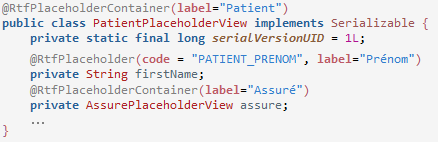
\includegraphics[width=11cm]{./img/annotations1}
  \caption{\label{fig:annotations} La classe PatientAnnotationView a été annotée avec 2 annotations (RtfPlaceholderContainer et RtfPlaceholder) afin de pouvoir être ensuite introspectée et servir à créer l'arborescence de placeholders.}
\end{figure}

\textbf{Pour comparer les deux solutions :} en terme de co\^ut, la première approche bénéficie d'un accés direct à l'information, mais celle-ci requiert un accés à la base de données et la reconstruction de l'arbre. Dans la deuxième approche, l'accés à l'information n'est pas direct, il faut parcourir les classes (couteux) et également reconstruire l'arborescence, mais on évite un accés à la base de données.\\
En ce qui concerne la maintenabilité, la deuxième solution est meilleure, surtout pour le lien entre le placeholder et la notation pointée.\\
Finalement, c'est donc la deuxième solution qui a été retenue et que j'ai implémentée.


\subparagraph*{Le remplacement des placeholders par leur valeur}
Le remplacement des placeholders par leur valeur a lieu lors de la sauvegarde du document, ou lorsque l'utilisateur demande une prévisualisation.\\

Trouver des expressions tokenisées dans un texte et les remplacer par leur valeur est une opération courante et de nombreuses bibliothèques ou objets permettent de le faire (Velocity, Freemaker, Antlr StringTemplate, StrSubstitutor etc.).
La bibliothèque Velocity étant déjà inclue dans le projet, c'est ce choix qui a été retenue.\\

Le remplacement des placeholders se fait en 3 phases : \\

\textbf{La phase 1} sert à remplacer les noms des placeholders par la notation pointée.\\
Cette phase se déroule en deux étapes : \\
D'abord, les classes java correspondant aux placeholders utilisés dans le texte sont parcourues pour remplir un contexte. Le contexte consiste en un dictionnaire de clés-valeurs, avec en clé le nom du placeholder et en valeur, la notation pointée.\\
Ensuite, \textit{Velocity} se sert du contexte pour remplacer les noms des placeholders par leur valeur.\\
%\begin{figure}[H]
%  \color{darkgray} 
%  \centering
%  $\$PATIENT\_NOM$ $~~~~~~~~$  => $\$patient.lastName$\\
%  $\$PATIENT\_ADRESSE2$  => $\$patient.address2$
%  \caption{\color{black} \label{fig:annotations} La phase 1 remplace le code du placeholder par la notation pointée qui y est associée.}
%\end{figure}

\textbf{La phase 2} sert à remplacer les notations pointées par leur valeur réelle.\\
Durant cette phase, on fait appel à l'API REST pour récupérer les objets métiers nécessaires, remplis avec les informations de la base de données.\\
Avec les objets métiers on remplit un nouveau contexte clé-valeur, avec en clé le nom de l'objet (première partie de la notation pointée) et en valeur l'objet lui même.\\
Ensuite, on refait appel à Velocity pour remplacer les notations objet par leur valeur.\\
%\begin{figure}[H]
%  \color{darkgray} 
%  \centering
%  $\$patient.lastName$ => $DUPONT$ $~~~~~~~~$\\
%  $\$patient.address2~$ => $\$patient.address2$ 
%  \caption{\color{black} \label{fig:annotations} La phase 2 remplace la notation pointée par la valeur en base. Si la valeur en base est "null", la notation pointée n'est pas remplacée.}
%\end{figure}

\textbf{La phase 3} sert à remplacer les valeurs non trouvées par des points d'interrogation.\\
En effet, lorsque \textit{Velocity} ne trouve pas une valeur, ou que la valeur est "null", il ne remplace pas la notation pointée.\\
Dans un soucis de propreté et également pour signifier à l'utilisateur que le remplacement n'a pas fonctionné, on insert une série de points d'interrogation.

%\begin{figure}[H]
%  \color{darkgray} 
%  \centering
%  $\$patient.address2$ => $???$
%  \caption{\color{black} \label{fig:annotations} La phase 3 remplace les notations pointées restantes par des points d'interrogation.}
%\end{figure}

\begin{figure}[H]
	\color{darkgray} 
	\centering
$\$PATIENT\_NOM$ $~~$ =1=> $\$patient.lastName$ =2=> $DUPONT$ $~$ =3=> $DUPONT$ $~$\\ $~$\\
  $\$PATIENT\_ADRESSE2$  =1=> $\$patient.address2$ =2=> $\$patient.address2~$ =3=> $???$ 	
	
	\caption{\color{black} \label{fig:annotations} Cette figure illustre la succession des 3 phases lors du remplacement d'un placeholder par sa valeur. Durant le processus, le placeholder est remplacé par la notation pointée, puis par sa valeur. Le deuxième exemple illustre le cas où aucune valeur n'a été trouvée en étape 2.}
\end{figure}

%TODO schéma récapitulatif : automate ?

%TODO : Remplacement des valeurs par les placeholders

%TODO Recap global de tout le truc : placeholder -> Valeur -> Placeholder
% Accés base, introspection des classes java, 3 phases, insertion du texte en js <-/-> Utilisation data-... + js pour value > placeholder

\subsubsection{Les modèles de texte}
La fonctionnalité des modèles de texte consiste à pouvoir sauvegarder dans une hiérarchie de dossiers, des documents RTF pouvant contenir des emplacements paramétrés.\\
Cette fonctionnalité se base sur la réutilisation de plusieurs autres :
\begin{itemize}
\item Le gestionnaire de fichiers et les hiérarchies de dossiers/fichiers.
\item Les documents texte.
\item Les placeholders.
\end{itemize}

%\subsubsection{Documents audio}
%\paragraph*{Web RTC}
%\paragraph*{Choix librairie front-end}
%\paragraph*{Intégration}

%TODO dire que c'est une feature secondaire, prévue pour plus tard.
		
\subsubsection{Introduction du concept de poste utilisateur dans le driver Pyvital}
\paragraph*{Motivations\\}
Au départ, le driver était uniquement conçu pour interragir avec le lecteur Sésam-Vitale.\\ Il avait alors été décidé que les websockets utilisées entre \textit{Sésame} et Pyvital aient pour identifiant le numéro de CPS\footnote{CPS: Carte de Professionnel de Santé} et la clé de licence.\\
%Néanmoins, il arrive que le logiciel soit utilisé par des auxiliaires médicales qui doivent effectuer des opérations pour plusieurs médecins. Dans ce cas de figure, il est peut judicieux de leur imposer de posséder les cartes de tous les praticiens. \\
Cependant, il a ensuité été prévu que le driver soit étendu pour supporter les opérations liées au scanner. Hors, pour cette fonctionnalité, il n'est pas nécessaire de disposer d'une CPS.\\
Pour ces raisons, nous avons décidé (avec mon chef de projet), de prendre pour nouvel identifiant de la websocket, le poste utilisateur (device) et la clé de licence. 

\paragraph*{Impact de la modification\\}
L'introduction du concept de poste utilisateur impacte la connexion de l'utilisateur à Topaze Web, et les communications entre Sesame et Pyvital.\\
Chaque utilisateur de Topaze peut être membre de plusieurs cabinets. Pour chaque cabinet, l'utilisateur dispose d'une licence Sesame lui autorisant l'usage de 3 postes utilisateurs. Lorsqu'il change de cabinet, l'utilisateur doit également choisir le poste utilisateur avec lequel ils souhaite se connecter à Sesame.\\

Lors de l'ajout de la fonctionnalité, de nombreux services de Topaze et Sesame ont étés impactés, ainsi que le driver Pyvital.
%TODO cf annexes.

\paragraph*{Sauvegarde des préférences utilisateurs\\}
Afin de ne pas re-demander à l'utilisateur de choisir un poste utilisateur à chaque connexion, il lui est permis d'enregistrer ses préférences.\\
Pour l'enregistrement des préférences, j'uilise un cookie qui stocke du json chiffré. Les clés du JSON sont les identifiants du couple Utilisateur-Cabinet et les valeurs sont les ids des postes utilisés dans chaque cas.

%%TODO schéma d'une requête de scan par exemple ? avec connexion puis scan.
%%TODO Faire le lien entre cabinetMember et device + possibilité de partager 1 device entre plusieurs cabinetMember + possiblité d'avoir 3 devices par licence.

%%TODO : Cookies pour stocker les devices + interfaces de choix.

%%TODO schéma du modèle, avant et après.

%De ce choix, il résulte une utilisation plus souple du logiciel (plus nécessairement besoin d'une CPS) et la possibilité de monayer plus facilement le logiciel (ex: possibilité de limiter le nombre de postes utilisateurs par licence).


\subsubsection{Les scans d'ordonnances}
\paragraph*{Fonctionnalité de numérisation\\}
Dans le dossier médical, l'utilisateur doit pouvoir ajouter des scans d'ordonnance (appelés SCOR\footnote{SCOR: SCannérisation des ORdonnances}).

\subparagraph*{Faisabilité}
Pour cette fonctionnalité, j'ai évalué qu'il était faisable de reproduire intégralement la fonctionnalité de Topaze Maestro.\\

La faisabilité de la fonctionnalité repose sur plusieurs éléments :\\
Dans un premier temps, il faut être capable de communiquer avec des scanners de différentes marques. Ceci est faisable grâce à l'interface de programmation et protocole de communication \textit{"TWAIN"}. Ce protocole permet de communiquer avec les drivers de  scanners à condition qu'ils implémentent l'API.\\
TWAIN a été créé en 1992\cite{bib:twain}, et la plupart des constructeurs font aujourd'hui partie du TWAIN groupe (HP, Adobe, Epson, Kodak, Fujitsu, Logitech etc.).\\
En python (langage du driver de Topaze Web), le module Pytwain permet d'interragir avec les scanners.\\

Ensuite, la fonction de scan de Topaze Maestro propose différentes options de scan (qualité, résolution, format de sortie, couleurs). Pour réaliser ces différentes options, il est possible d'utiliser la bibliothèque \textit{Pillow} qui permet de réaliser différent traitements de l'image (conversion de couleurs, redimensionnement, encodage etc.)\cite{bib:pillow}.\\

D'autre part, Topaze Maestro propose une interface graphique permettant d'appliquer différents traitements à l'image numérisée (cropping, redimensionnement, rotation). 
Pour réaliser ces fonctionnalités, il existe de nombreuses possibilités. On peut par exemple le faire entièrement coté navigateur, au moyen d'une bibliothèque javascript (il en existe plusieurs). Soit opter pour une solution hybride. Dans ce cas, il est par exemple possible de faire une prévisualisation en javascript, et le traitement en Python avec Pillow. 
Enfin, le dernier choix consiste à faire la prévisualisation en javascript coté client et le traitement en java, coté serveur. \\

Enfin, il est nécessaire de faire communiquer le driver avec le serveur Sésame. Ce problème a déja été entièrement résolu avant mon arrivée.
%TODO annexe : interfaces de scan dans topaze Maestro et Web.

\paragraph*{Implémentation du scan d'images}
% Parler de l'implem avec twain : définition de la taille d'image + params (résolution (dpi), quality, Noir/blanc + acquire, callback, récupération de l'image, conversion dans le format d'image souhaité avec Pillow, respect des dpi avec Pillow, retour à Sésame grâce aux websocket définies précédemment.
%TODO inclure schéma de séquence
\subparagraph*{Fonctionnement global}
La fonctionnalité de numérisation fait intervenir les serveurs Topaze Webapp, TopazeRest et Sésame ainsi que le driver Pyvital qui se trouve sur le poste client.
Sur chaque serveur ou client, différents composants interviennent :
\begin{figure}[H]
  \centering
  \includegraphics[width=16cm]{./img/macro_sesame3}
  \caption{\label{fig:mb_va_ast} Diagrame UML de déploiement représentant les différents composants qui interviennent lors d'une requête au scanner.}
\end{figure}

\subparagraph*{Déroulement d'une demande de numérisation}
Dans un premier temps, un utilisateur clique sur le bouton "numériser" de l'application web. À ce moment, une méthode est appeléée sur l'un des controlleurs de Topaze Webapp. Le controleur va ensuite contacter le serveur Topaze Rest qui sert ici de proxy avec le serveur Sesame. \\
Le composant Topaze Rest met à disposition un controlleur qui relie une URL publique à un service. Topaze Rest-Client permet de contacter le controleur de topaze Rest via l'appel d'une méthode. Ce mécanisme permet ainsi à Topaze WebApp d'utiliser les services de Topaze Rest en toute transparence. \\
Dans la suite du processus, le serveur Topaze Rest contacte Sesame Rest. \\
Le serveur Sesame Rest est doté du même mécanisme que sur Topaze, mais il dispose en plus de deux autres composants lui permettant de contacter le driver Pyvital.\\
Le composant Sesame-Repository contient un "driver distant" qui traite les actions spécifiques au scanner. Sesame WebSocket permet quant à lui de gérer la communication en websockets avec le driver Pyvital.\\
Enfin, le driver \textit{Pyvital} utilise TWAIN pour réaliser l'acquisition d'image avec le scanner.\\

Mon travail lors de l'implémentation de la fonctionnalité a été créer les services nécessaires sur Topaze et Sesame et d'ajouter la fonction de numérisation sur Pyvital.

\subparagraph*{Communication entre Sesame et Pyvital}
Pour que Sesame puisse demander à Pyvital d'effectuer des actions, il nécessaire d'implémenter certaines interfaces. Il faut par exemple implémenter un MessagePreparator et un MessageHandler ainsi que les fabriques associées. Ces classes seront chargées de préparer le message transmis à Pyvital de traiter la réception des messages qui en proviennent. \\

L'enchainement des actions est résumé sur le diagramme de séquence suivant :

\begin{figure}[H]
  \centering
  \includegraphics[width=17cm]{./img/diag_seq_sesame}
  \caption{\label{fig:diag_seq_sesame} Diagrame de séquence illustrant la communication entre Sesame et Pyvital.}
\end{figure}

\subparagraph*{La numérisation sur Pyvital}
Sur Pyvital, j'ai utilisé TWAIN afin de réaliser la numérisation des documents. Le scan d'un document se déroule en plusieurs étapes. Dans un premier temps, on demande à Twain de lancer l'acquisition de données. Une fois l'acquisition réalisée, un callback est appelé afin de permettre l'obtention de l'image. Puis, des traitements sont effectués sur l'image (résolution, qualité, couleur etc.), grâche à Pillow. Enfin, l'image est convertie en Base64 et transmise à Sésame via les websockets.
 
\begin{figure}[H]
  \centering
  \includegraphics[width=17cm]{./img/numerisation}
  \caption{\label{fig:diag_seq_sesame} Diagrame d'activités UML représentant les différentes étapes effectuées par Pyvital, lors d'une demande de numérisation.}
\end{figure}

%\paragraph*{Traitement d'image (cropping/rotation/zoom)\\}
%TODO
%TODO parler de l'intégration de l'outil .... 

%\paragraph*{Génération d'un pdf\\}
%TODO
%TODO coté front car économie coux serveur  + fallback coté java/back pour Android car non available.
		
\subsubsection{Installateur Windows pour le driver}
Ayant travaillé sur le driver python et dans l'objectif d'une commercialisation qui approche, il m'a été demandé de réaliser un installateur windows pour le driver.

\paragraph*{Fonctionnalités de l'installateur\\}
Le rôle de l'installateur est double.\\ 
La première fois qu'il est exécuté, son but est d'installer Pyvital et de créer un nouveau poste utilisateur (à la fois sur le driver et en base de donnée). \\
Toutes les autres fois ou l'installateur est appelé, il ne sert qu'à lier de nouvelles clés de licence au poste utilisateur.\\

Par exemple, si un utilisateur exerce dans deux cabinets, il doit lancer l'installateur une première fois pour installer Pyvital et lier son compte (sur le premier cabinet) au nouveau poste utilisateur.
Si il souhaite également lier son compte sur le deuxième cabinet, il doit relancer l'installateur. La deuxième fois, l'installateur ne fera que lier la clé de licence (associée au couple Utilisateur-Cabinet) au poste existant.

Cet enchaînement d'action est décrit dans le schéma ci-dessous : 
\begin{figure}[H]
  \vspace{-10pt}
  \centering
  \includegraphics[width=17cm]{./img/installateur}
  \caption{\label{fig:installateur} Diagrame d'activités UML représentant les deux modes de l'installateur..}
\end{figure}

\paragraph*{Installation de Pyvital}
Lors de l'installation de Pyvital, l'installateur doit déplacer les fichiers du driver dans le bon dossier sur windows. Puis, il doit installer les dépendances et les .msi nécessaires.\\ 
Il doit également compléter le fichier de configuration du driver. \\
Ensuite, il doit contacter le serveur \textit{Sésame} afin de vérifier la clé de licence et d'enregistrer le nouveau poste utilisateur. \\
Enfin, il doit installer le logiciel Pyxvital qui est utilisé pour les opérations de facturation liées au lecteur Sésam.

\paragraph*{Choix de la solution technique\\}
Pour le choix de l'installateur, la solution d'\textit{Inno Setup} m'a été recommandée par le directeur de l'entreprise. En effet, il s'agit de la solution qui est utilisée dans les dernières versions de Topaze Maestro.\\
Avant d'opter définitivement pour Inno Setup, j'ai vérifié que l'installateur recommandé satisfasse les exigences du projet.\\ Lors de l'installation, il fallait par exemple que je puisse installer des .msi\footnote{MSI: Microsoft Installer} en mode silencieux. Il fallait aussi que je puisse ajouter des écrans supplémentaires lors de l'installation. Enfin, je devais pouvoir effectuer des requêtes HTTP vers notre serveur Sésame.

\paragraph*{Implémentation\\}
Inno Setup est un outil qui permet de réaliser simplement des installateurs. L'outil prend en charge la création des interfaces graphiques et d'une partie des opérations standards (ex: déplacements de fichiers). Pour l'utiliser, on remplit un fichier \textit{.iss}\footnote{.ISS: Inno Setup Script} qui permet de configurer l'installateur et d'étendre ses fonctionnalités. Le fichier .iss est structuré en sections et chaque section permet de décrire de façon déclarative la façon dont l'installateur doit se comporter. Les sections principales sont : 
\begin{sitemize}
\item Setup : section qui décrit le nom du programme, sa version, son dossier d'installation etc.
\item Dirs : les dossiers à créer.
\item Files : les fichiers à déplacer (avec leur source et leur destination).
\item Icons : les raccourcis à créer dans le menu démarrer ou sur le bureau.
\item Ini : les variables à initialiser dans le fichier \textit{.ini} de l'application.
\item Run : le programme à lancer lorsque l'installation est finie.
\item Code : la partie qui permet d'étendre inno setup au moyen de code pascal.
\item d'autres sections moins importantes : types (les types d'installations), components (des groupes de tâches), tasks, languages, installDelete, uninstallDelete, uninstallRun, registry etc.
\end{sitemize}  

Dans l'installateur, la partie la plus importante est la section \textit{"Code"} car elle permet d'ajouter des écrans à l'installateur et de créer de nouvelles fonctionnalités. Sur le projet, je l'ai utilisé pour créer une page de validation de clé de licence, et une page servant à définir le nom du nouveau poste utilisateur.\\
Dans ces deux cas, l'installateur réalise une requête HTTP vers le serveur Sésame, puis traite la réponse obtenue. 

\paragraph*{L'intégration de pixvital\\}
%Pyxvital est un logiciel qui sert à créer des FSE\footnote{FSE: Feuille de Soins Electroniques} et à assurer la transmission avec le lecteur Sésam-Vitale. Il est utilisé temporairement afin de faciliter la certification de Topaze Web et accélerer ainsi sa mise sur le marché.
%TODO : Hors sujet. ^

Le driver de Topaze Web utilise Pixvital et il est donc nécessaire que celui-ci soit installé en même temps que les autres dépendances. Le problème de Pixvital est qu'il ne peut être installé qu'au moyen d'un \textit{.exe}. Hors, nous souhaitons que son installation soit transparante pour l'utilisateur. Il a donc été nécessaire de comprendre les différentes opérations réalisées lors de l'installation, afin de les inclure dans notre installateur.\\
Pour ce faire, j'ai donc du lancer l'installateur de Pixvital et regarder si des registres étaient modifiés, quels fichiers étaient installés et quels fichiers de configuration étaient complétés. Ensuite, j'ai dû ajouter ces opérations à la phase finale d'installation dans Inno Setup.


\subsection{Protocole d'évaluation}
\subsubsection{Evaluation de la qualité du code}
\paragraph*{Tests unitaires\\}
Pour s'assurer de la qualité du logiciel, nous effectuons des tests unitaires JUnit sur les services réalisés, les composants métiers et tout ce qui contient de la logique métier. Ces tests permettent également de garantir la non-régression du code.

\paragraph*{Le développement dirigé par les tests\\}
Les tests unitaires sont dans la mesure du possible réalisés en respectant la méthodologie du Test Driven Development.\\
La méthode de développement dirigé par les tests a été progressivement mise en place lors du sprint 2 et permet de garantir une meilleure qualité du code. En effet, par l'utilisation de cette méthode, on est certain que chaque fonctionnalité a été testée. D'autre part, chaque test sert en quelques sortes de spécification pour le morceau de code testé.

\paragraph*{L'intégration continue et l'inspecteur de qualité de code\\} 
Durant le sprint 2, un serveur d'intégration continue a été mis en place. Pour ce faire, un membre de l'équipe a déployé un serveur Jenkins. De ce fait, les tests unitaires sont désormais lancés à chaque build. \\
Par la suite, SonarQube a également été installé. Il s'agit d'un outil réalisant l'inspection de la qualité de code. Il fournit une estimation de la dette technique et pointe les problèmes rencontrés. Il fournit également une explication détaillée pour chaque problème rencontré.

\paragraph{Revues de code\\}
Fréquemment, le chef de projet effectue des revues de code et peut demander à ce que certaines parties soient re-factorisées ou que l'architecture soit revue.

\subsubsection{Evaluation fonctionnelle du logiciel}
\paragraph*{Les réunions avec le client en fin de sprint\\}
À la fin de chaque sprint, une réunion de démonstration est organisée avec le client. C'est alors le moment d'avoir son retour sur les fonctionnalités développées. Cette réunion peut donner lieu à des rectifications à réaliser si le besoin a été mal compris ou si des évolutions sont souhaitées. \\
%Le client étant la société soeur de Supralog, nous disposons d'un lien étroit avec elle. En effet, un membre d'IDEA est chargé de faire la liaison entre le projet Topaze Web et IDEA. Nous pouvons donc le consulter en cas de doûte sur les besoins ou sur la compréhension de l'attendu.

% Tests unitaires
% Satisfaction client